\usepackage{biblatex}\subsection{Dane wejściowe}
\label{subsec:dane-wejsciowe}

\subsubsection{Notacja Forsytha-Edwardsa}

Aby umożliwić komunikację z programem, należy w pierwszej kolejności sprecyzować, w jakim formacie dostarczone zostaną dane wejściowe reprezentujące konkretną pozycję szachową.
Standardem, wykorzystywanym nie tylko w większości silników, ale także w pojedynkach rozgrywanych online, jest Notacja Forsytha-Edwardsa (ang.~\emph{Forsyth–Edwards~Notation}, w~skrócie FEN).
Jest to format stworzony specjalnie na potrzeby komputerów.
FEN pozwala na jednoznaczne określenie pozycji na szachownicy.
Przykład notacji dla pozycji startowej:

\vspace{5mm}
\centerline{
    \ref{fig: figure} a) \lstset{basicstyle=\ttfamily}\lstinline{rnbqkbnr/pppppppp/8/8/8/8/PPPPPPPP/RNBQKBNR w KQkq - 0 1}
}
\centerline{
    \ref{fig: figure} b) \lstset{basicstyle=\ttfamily}\lstinline{rnbqkbnr/pppppppp/8/8/4P3/8/PPPP1PPP/RNBQKBNR b KQkq e3 0 1}
}
\vspace{5mm}

\begin{figure}[htb]
    \centering
    \begin{tabular}{@{}ll@{}}
        a) & b) \\
        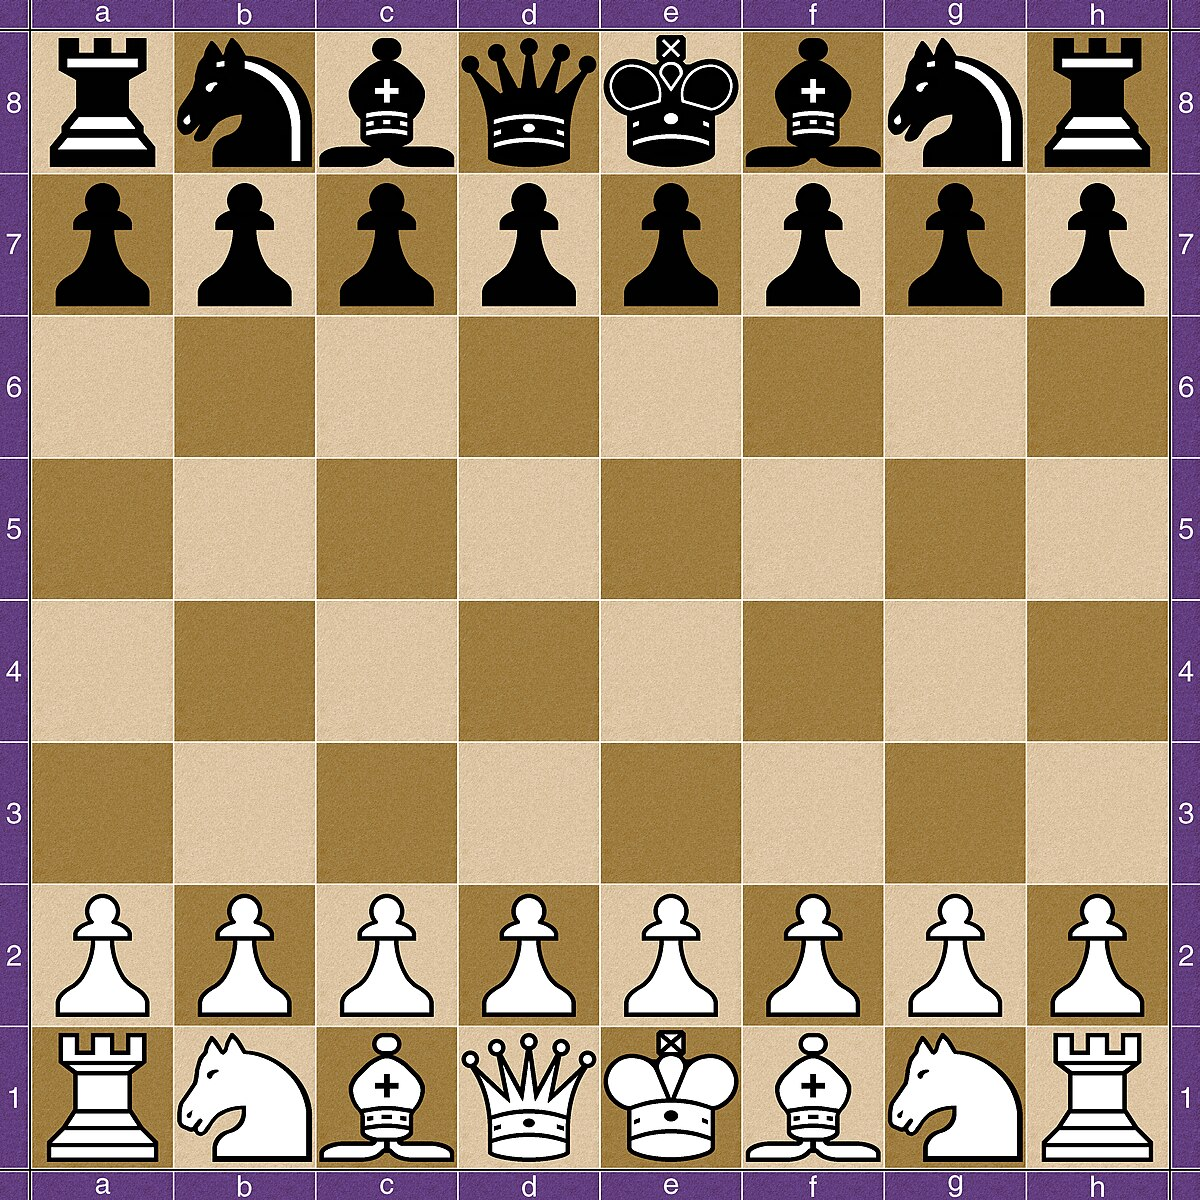
\includegraphics[width=0.475\textwidth]{rozdzialy/rozdzial01/1_uniwersalny-interfejs-szachowy/rysunki/pozycja_startowa}
        &
        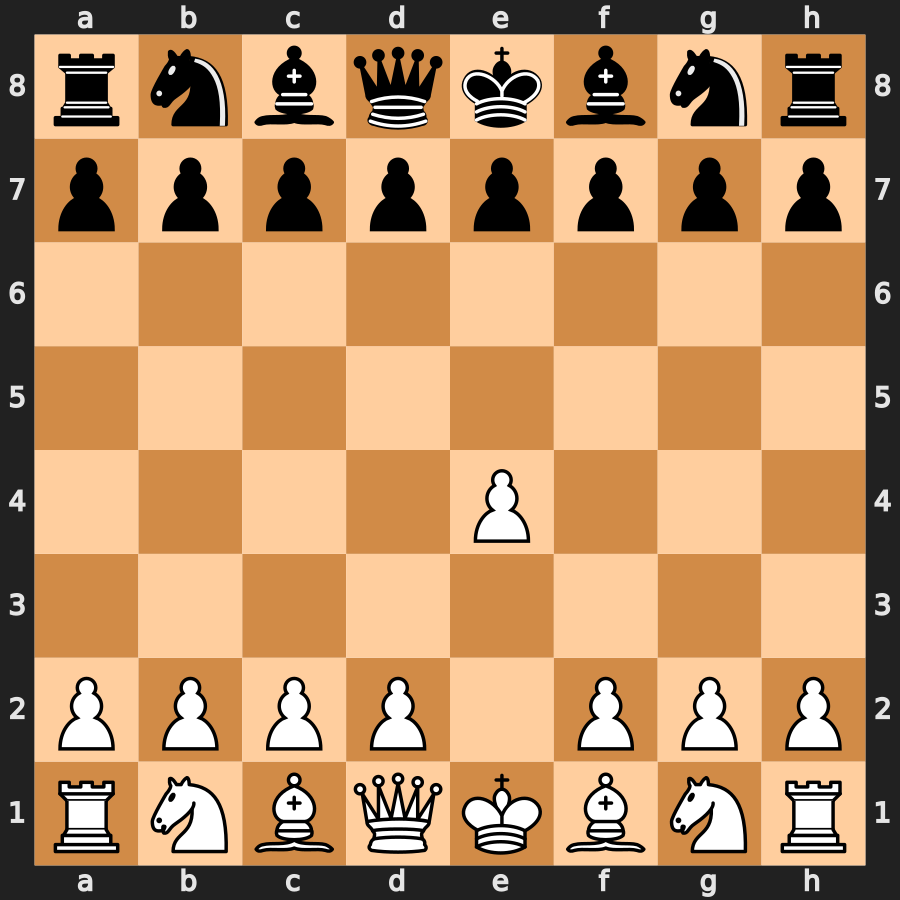
\includegraphics[width=0.475\textwidth]{rozdzialy/rozdzial01/1_uniwersalny-interfejs-szachowy/rysunki/pozycja_startowa_e2e4}
    \end{tabular}
   \caption{Przykładowce pozycje szachowe: a) startowa, b) po ruchu e2e4}
    \label{fig: figure}
\end{figure}

Całość informacji, zawartych w jednej linii znaków kodowanych ASCII, ma 6 pól oddzielonych spacjami.
Pola te informują, o różnych aspektach danej pozycji:

\begin{enumerate}
    \item Reprezentacja 64 pól szachownicy.
    Każdy z wierszy szachownicy oddzielony jest ,,/''.
    Odpowiednio dla białych i czarnych figur.
    \item Czyj jest ruch (w — białe, b — czarne)
    \item Możliwości roszady (K/k — krótka roszada, Q/q — długa roszada)
    \item Możliwości bicia w przelocie, znanego szerzej jako ruch en passant.
    Sprecyzowane pole jest polem atakowanym.
    W przypadku braku możliwości bicia w przelocie w polu widnieje ,,-''.
    \item Liczba posunięć od ostatniego bicia bądź ruchu pionem.
    Istotna w regule 50 posunięć.
    \item Liczba pełnych ruchów.
\end{enumerate}

\subsubsection{Szachowa notacja algebraiczna}
Przykład odniesienia do bibliografii\cite{knuth1990, greenwade1993}.
Udało się?